\chapter{Discussion and Results}

\section{Results}

    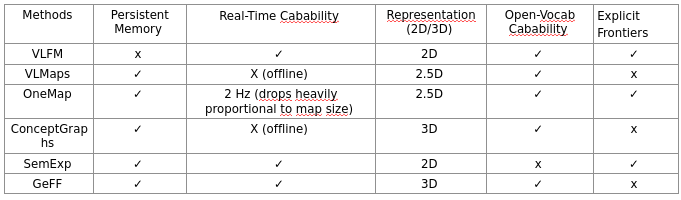
\includegraphics[width=\textwidth]{Images/1_introduction/temp_sota_comparison_common_properties.png}

    All \(\boldsymbol{GP}_{\text{models}}\) are tested against the ground truth sensor measurement while live predicting. The results are structured in the results of the \(\boldsymbol{GP}_{\text{effort}}\) models for both datasets \(\mathcal{D}_{\text{Cartesian}}\) and \(\mathcal{D}_{\text{CartesianOC}}\) and in the results of the \(\boldsymbol{GP}_{\text{wrench}}\) for both datasets \(\mathcal{D}_{\text{Cartesian}}\) and \(\mathcal{D}_{\text{CartesianOC}}\). 
    After that the serial prediction of both \(\boldsymbol{GP}_{\text{models}}\) is estimation the resulting f/t measurements at the measurement frame. The estimation is the subtracted from the actual measurements to evaluate how accurate the \(\boldsymbol{GP}_{\text{models}}\) isolate the f/t measurement resulting from the gripper. In this case the both best performing \(\boldsymbol{GP}_{\text{models}}\) of each dataset \(\mathcal{D}_{\text{Cartesian}}\) and \(\mathcal{D}_{\text{CartesianOC}}\) are chosen and the isolation accuracy is evaluated for both trajectory patterns with and without orientation change. 

    \subsection{Results \(\boldsymbol{GP}_{\text{effort}}\) model}
    \label{subsec:gp_effort_results}

    \begin{figure}[H]
    \centering
    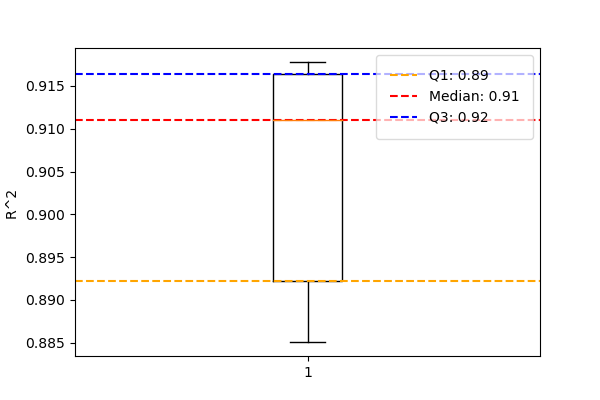
\includegraphics[width=1\columnwidth]{Images/05_results/effort_boxplot_test_non_OC_R^2.png}
    \caption[\(\boldsymbol{GP}_{\text{effort}}\) model \(R^2\) on effort \(\mathcal{D}_{\text{Cartesian}}\) test data]{\(\boldsymbol{GP}_{\text{effort}}\) model \(R^2\) on effort \(\mathcal{D}_{\text{Cartesian}}\) test data}
    \label{fig:effort_no_oc_R^2_test}
    \end{figure}

    \begin{figure}[H]
    \centering
    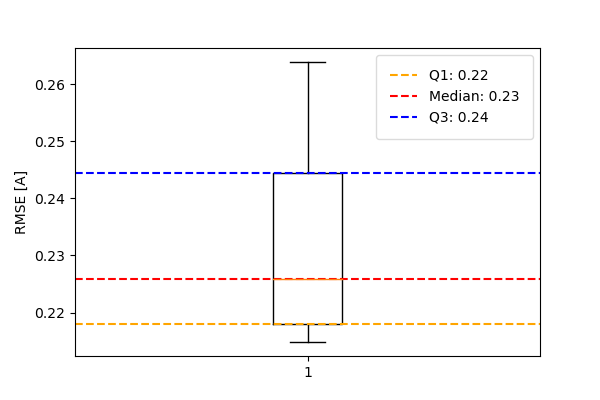
\includegraphics[width=1\columnwidth]{Images/05_results/effort_boxplot_test_non_OC_RMSE.png}
    \caption[\(\boldsymbol{GP}_{\text{effort}}\) model \(RMSE\) on effort \(\mathcal{D}_{\text{Cartesian}}\) test data]{\(\boldsymbol{GP}_{\text{effort}}\) model \(RMSE\) on effort \(\mathcal{D}_{\text{Cartesian}}\) test data}
    \label{fig:effort_no_oc_RMSE_test}
    \end{figure}
    
    
    \begin{table}[H]
    \centering
    \begin{tabular}{lcccc}
    \toprule
    \textbf{Model} & \textbf{MAE} & \textbf{MSE} & \textbf{RMSE} & \textbf{R\textsuperscript{2}} \\
    \midrule
    Model\_1 & 0.1284 & 0.1207 & 0.2639 & 0.8851 \\
    Model\_2 & 0.1186 & 0.1190 & 0.2556 & 0.8868 \\
    Model\_3 & 0.1134 & 0.1196 & 0.2496 & 0.8863 \\
    Model\_4 & 0.1141 & 0.0953 & 0.2286 & 0.9093 \\
    Model\_5 & 0.1098 & 0.0964 & 0.2287 & 0.9083 \\
    Model\_6 & 0.1080 & 0.0876 & 0.2179 & 0.9166 \\
    Model\_7 & 0.1100 & 0.0918 & 0.2232 & 0.9127 \\
    Model\_8 & 0.1071 & 0.0867 & 0.2154 & 0.9175 \\
    Model\_9 & 0.1077 & 0.0885 & 0.2182 & 0.9158 \\
    Model\_10 & 0.1070 & 0.0864 & 0.2148 & 0.9178 \\
    \bottomrule
    \end{tabular}
    \caption{\(\boldsymbol{GP}_{\text{effort}}\) model metrics on effort \(\mathcal{D}_{\text{Cartesian}}\) test data}
    \end{table}

    \begin{figure}[H]
    \centering
    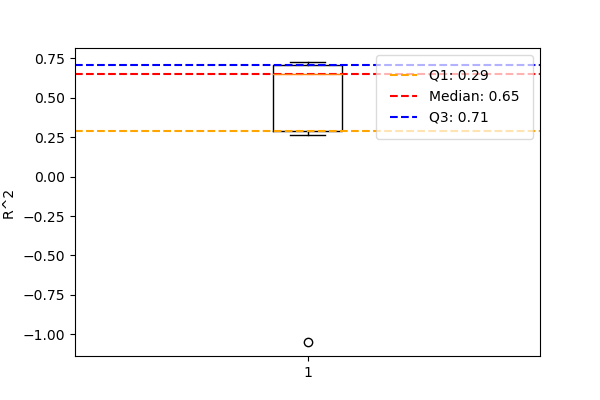
\includegraphics[width=1\columnwidth]{Images/05_results/effort_boxplot_live_non_OC_R^2.png}
    \caption[\(\boldsymbol{GP}_{\text{effort}}\) model \(R^2\) on effort Cartesian trajectories without orientation change live prediction]{\(\boldsymbol{GP}_{\text{effort}}\) model \(R^2\) on effort Cartesian trajectories without orientation change live prediction}
    \label{fig:effort_no_oc_R^2_live}
    \end{figure}

    \begin{figure}[H]
    \centering
    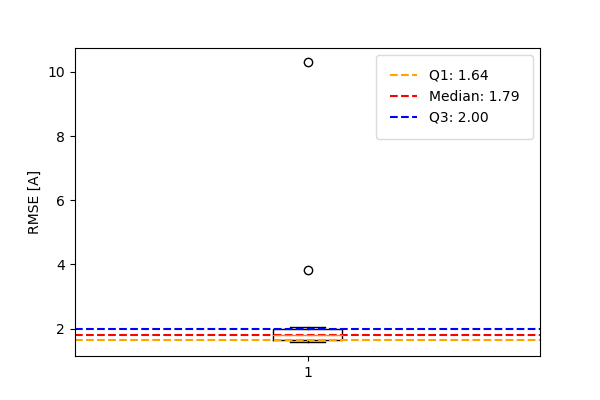
\includegraphics[width=1\columnwidth]{Images/05_results/effort_boxplot_live_non_OC_RMSE.png}
    \caption[\(\boldsymbol{GP}_{\text{effort}}\) model \(RMSE\) on effort Cartesian trajectories without orientation change live prediction]{\(\boldsymbol{GP}_{\text{effort}}\) model \(RMSE\) on effort Cartesian trajectories without orientation change live prediction}
    \label{fig:effort_no_oc_RMSE_live}
    \end{figure}
    
    \begin{table}[H]
    \centering
    \begin{tabular}{lcccc}
    \toprule
    \textbf{Model} & \textbf{MAE} & \textbf{MSE} & \textbf{RMSE} & \textbf{R\textsuperscript{2}} \\
    \midrule
    Model\_1 & 0.9905 & 3.8876 & 1.6011 & 0.7277 \\
    Model\_2 & 1.0559 & 4.8169 & 1.7499 & 0.6838 \\
    Model\_3 & 0.9799 & 4.2983 & 1.6435 & 0.6163 \\
    Model\_4 & 7.0056 & 219.6050 & 10.3051 & -1.0499 \\
    Model\_5 & 1.0073 & 5.1650 & 1.8236 & 0.7022 \\
    Model\_6 & 0.9912 & 3.7223 & 1.5833 & 0.7136 \\
    Model\_7 & 1.0880 & 5.6405 & 1.8270 & 0.3171 \\
    Model\_8 & 1.6480 & 31.9329 & 3.8415 & 0.2818 \\
    Model\_9 & 0.9942 & 4.1817 & 1.6450 & 0.7131 \\
    Model\_10 & 1.2684 & 7.4675 & 2.0570 & 0.2626 \\
    \bottomrule
    \end{tabular}
    \caption{\(\boldsymbol{GP}_{\text{effort}}\) model live prediction metrics on effort Cartesian trajectories without changing orientation}
    \end{table}

    
    \begin{figure}[H]
    \centering
    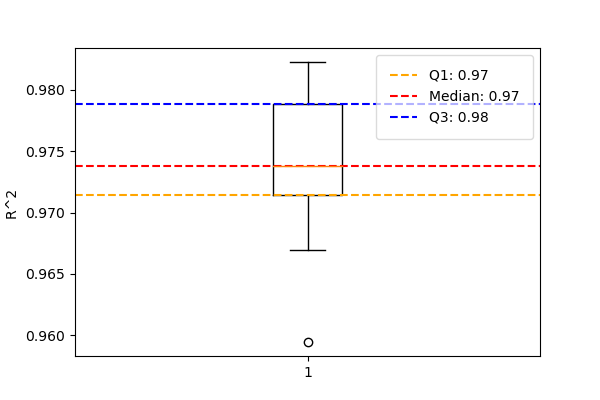
\includegraphics[width=1\columnwidth]{Images/05_results/effort_boxplot_test_OC_R^2.png}
    \caption[\(\boldsymbol{GP}_{\text{effort}}\) model \(R^2\) on effort \(\mathcal{D}_{\text{CartesianOC}}\) test data]{\(\boldsymbol{GP}_{\text{effort}}\) model \(R^2\) on effort \(\mathcal{D}_{\text{CartesianOC}}\) test data}
    \label{fig:effort_oc_R^2_test}
    \end{figure}

    \begin{figure}[H]
    \centering
    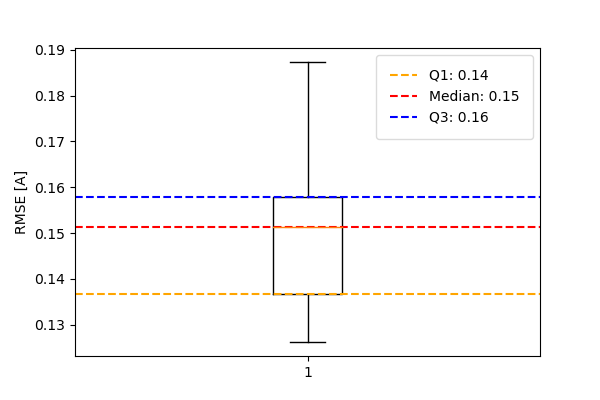
\includegraphics[width=1\columnwidth]{Images/05_results/effort_boxplot_test_OC_RMSE.png}
    \caption[\(\boldsymbol{GP}_{\text{effort}}\) model \(RMSE\) on effort \(\mathcal{D}_{\text{CartesianOC}}\) test data]{\(\boldsymbol{GP}_{\text{effort}}\) model \(RMSE\) on effort \(\mathcal{D}_{\text{CartesianOC}}\) test data}
    \label{fig:effort_oc_RMSE_test}
    \end{figure}

    \begin{table}[H]
    \centering
    \begin{tabular}{lcccc}
    \toprule
    \textbf{Model} & \textbf{MAE} & \textbf{MSE} & \textbf{RMSE} & \textbf{R\textsuperscript{2}} \\
    \midrule
    Model\_1 & 0.1156 & 0.0411 & 0.1873 & 0.9595 \\
    Model\_2 & 0.1076 & 0.0335 & 0.1700 & 0.9670 \\
    Model\_3 & 0.1034 & 0.0294 & 0.1590 & 0.9710 \\
    Model\_4 & 0.1008 & 0.0278 & 0.1548 & 0.9726 \\
    Model\_5 & 0.0942 & 0.0246 & 0.1460 & 0.9758 \\
    Model\_6 & 0.0989 & 0.0267 & 0.1514 & 0.9737 \\
    Model\_7 & 0.0984 & 0.0266 & 0.1511 & 0.9738 \\
    Model\_8 & 0.0851 & 0.0204 & 0.1335 & 0.9799 \\
    Model\_9 & 0.0802 & 0.0185 & 0.1277 & 0.9817 \\
    Model\_10 & 0.0793 & 0.0180 & 0.1262 & 0.9822 \\
    \bottomrule
    \end{tabular}
    \caption{\(\boldsymbol{GP}_{\text{effort}}\) model metrics on effort \(\mathcal{D}_{\text{CartesianOC}}\) test data}
    \end{table}

    \begin{figure}[H]
    \centering
    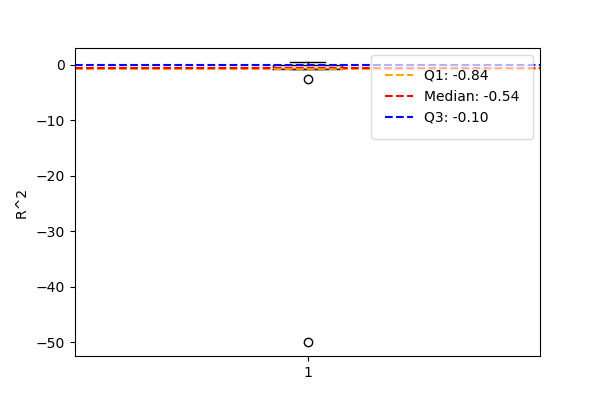
\includegraphics[width=1\columnwidth]{Images/05_results/effort_boxplot_live_OC_R^2.png}
    \caption[\(\boldsymbol{GP}_{\text{effort}}\) model \(R^2\) on effort Cartesian trajectories with orientation change live prediction]{\(\boldsymbol{GP}_{\text{effort}}\) model \(R^2\) on effort Cartesian trajectories with orientation change live prediction}
    \label{fig:effort_oc_R^2_live}
    \end{figure}

    \begin{figure}[H]
    \centering
    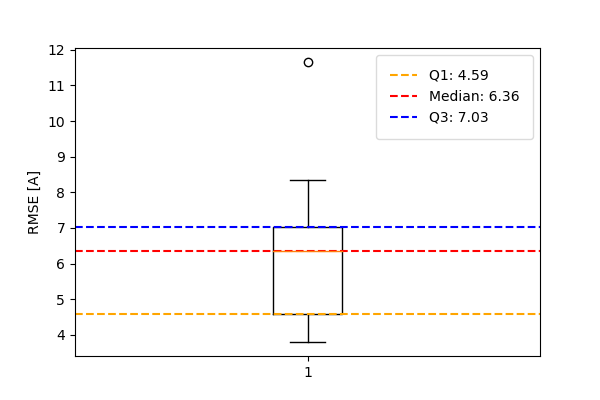
\includegraphics[width=1\columnwidth]{Images/05_results/effort_boxplot_live_OC_RMSE.png}
    \caption[\(\boldsymbol{GP}_{\text{effort}}\) model \(RMSE\) on effort Cartesian trajectories with orientation change live prediction]{\(\boldsymbol{GP}_{\text{effort}}\) model \(RMSE\) on effort Cartesian trajectories with orientation change live prediction}
    \label{fig:effort_oc_RMSE_live}
    \end{figure}

    \begin{table}[H]
    \centering
    \begin{tabular}{lcccc}
    \toprule
    \textbf{Model} & \textbf{MAE} & \textbf{MSE} & \textbf{RMSE} & \textbf{R\textsuperscript{2}} \\
    \midrule
    Model\_1 & 4.6183 & 44.5287 & 5.0202 & -49.9557 \\
    Model\_2 & 5.0939 & 84.8610 & 7.1296 & -0.8461 \\
    Model\_3 & 7.9057 & 170.7499 & 11.6557 & -2.6656 \\
    Model\_4 & 2.7165 & 21.7399 & 3.8019 & -0.4782 \\
    Model\_5 & 2.3954 & 22.5525 & 4.0519 & 0.4712 \\
    Model\_6 & 3.7646 & 65.8977 & 6.6115 & -0.0089 \\
    Model\_7 & 3.8694 & 48.5134 & 6.1077 & -0.3607 \\
    Model\_8 & 5.1302 & 59.7537 & 6.7226 & -0.8230 \\
    Model\_9 & 2.7820 & 23.8206 & 4.4423 & -0.0130 \\
    Model\_10 & 5.9914 & 86.0272 & 8.3497 & -0.6062 \\
    \bottomrule
    \end{tabular}
    \caption{\(\boldsymbol{GP}_{\text{effort}}\) model live prediction metrics on effort Cartesian trajectories with changing orientation}
    \end{table}


    \subsection{Results \(\boldsymbol{GP}_{\text{wrench}}\) model}
    \label{subsec:gp_wrench_results}

    \begin{figure}[H]
    \centering
    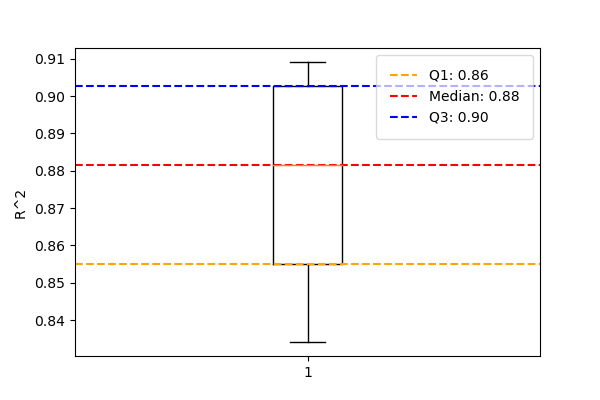
\includegraphics[width=1\columnwidth]{Images/05_results/wrench_boxplot_test_non_OC_R^2.png}
    \caption[\(\boldsymbol{GP}_{\text{wrench}}\) model \(R^2\) on wrench \(\mathcal{D}_{\text{Cartesian}}\) test data]{\(\boldsymbol{GP}_{\text{wrench}}\) model \(R^2\) on wrench \(\mathcal{D}_{\text{Cartesian}}\) test data}
    \label{fig:wrench_no_oc_R^2_test}
    \end{figure}

    \begin{figure}[H]
    \centering
    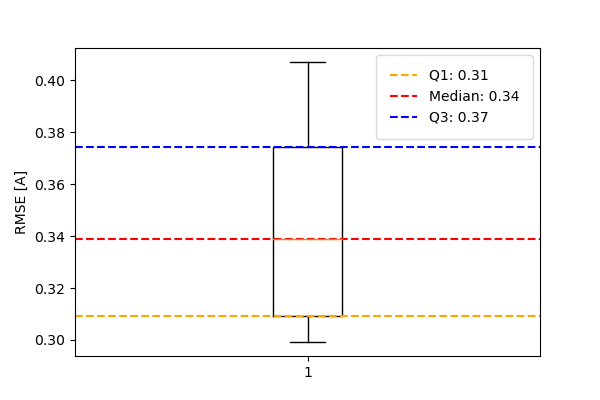
\includegraphics[width=1\columnwidth]{Images/05_results/wrench_boxplot_test_non_OC_RMSE.png}
    \caption[\(\boldsymbol{GP}_{\text{wrench}}\) model \(RMSE\) on wrench \(\mathcal{D}_{\text{Cartesian}}\) test data]{\(\boldsymbol{GP}_{\text{wrench}}\) model \(RMSE\) on wrench \(\mathcal{D}_{\text{Cartesian}}\) test data}
    \label{fig:wrench_no_oc_RMSE_test}
    \end{figure}


    \begin{table}[H]
    \centering
    \begin{tabular}{lcccc}
    \toprule
    \textbf{Model} & \textbf{MAE} & \textbf{MSE} & \textbf{RMSE} & \textbf{R\textsuperscript{2}} \\
    \midrule
    Model\_1 & 0.1670 & 0.1724 & 0.4070 & 0.8341 \\
    Model\_2 & 0.1441 & 0.1541 & 0.3778 & 0.8526 \\
    Model\_3 & 0.1521 & 0.1661 & 0.3919 & 0.8410 \\
    Model\_4 & 0.1458 & 0.1437 & 0.3636 & 0.8624 \\
    Model\_5 & 0.1304 & 0.1118 & 0.3223 & 0.8930 \\
    Model\_6 & 0.1264 & 0.0984 & 0.3047 & 0.9058 \\
    Model\_7 & 0.1249 & 0.0949 & 0.2996 & 0.9091 \\
    Model\_8 & 0.1254 & 0.0949 & 0.2992 & 0.9091 \\
    Model\_9 & 0.1349 & 0.1141 & 0.3273 & 0.8907 \\
    Model\_10 & 0.1361 & 0.1334 & 0.3502 & 0.8724 \\
    \bottomrule
    \end{tabular}
    \caption{\(\boldsymbol{GP}_{\text{wrench}}\) model metrics on effort \(\mathcal{D}_{\text{Cartesian}}\) test data}
    \end{table}

    \begin{figure}[H]
    \centering
    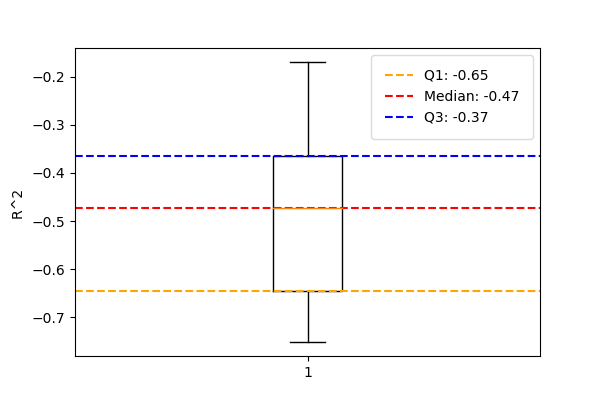
\includegraphics[width=1\columnwidth]{Images/05_results/wrench_boxplot_live_non_OC_R^2.png}
    \caption[\(\boldsymbol{GP}_{\text{wrench}}\) model \(R^2\) on wrench Cartesian trajectories without orientation change live prediction]{\(\boldsymbol{GP}_{\text{wrench}}\) model \(R^2\) on wrench Cartesian trajectories without orientation change live prediction}
    \label{fig:wrench_no_oc_R^2_live}
    \end{figure}

    \begin{figure}[H]
    \centering
    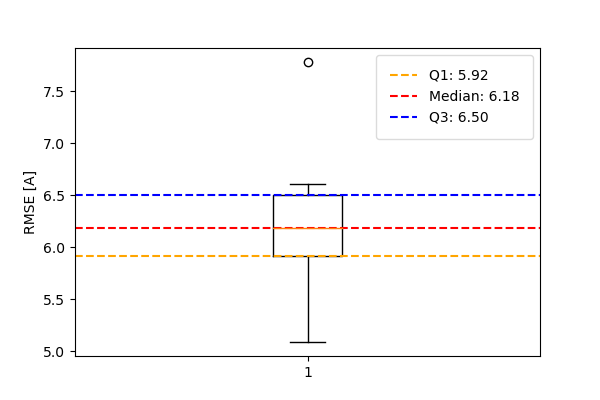
\includegraphics[width=1\columnwidth]{Images/05_results/wrench_boxplot_live_non_OC_RMSE.png}
    \caption[\(\boldsymbol{GP}_{\text{wrench}}\) model \(RMSE\) on wrench Cartesian trajectories without orientation change live prediction]{\(\boldsymbol{GP}_{\text{wrench}}\) model \(RMSE\) on wrench Cartesian trajectories without orientation change live prediction}
    \label{fig:wrench_no_oc_RMSE_live}
    \end{figure}

    
    \begin{table}[H]
    \centering
    \begin{tabular}{lcccc}
    \toprule
    \textbf{Model} & \textbf{MAE} & \textbf{MSE} & \textbf{RMSE} & \textbf{R\textsuperscript{2}} \\
    \midrule
    Model\_1 & 4.1511 & 67.9632 & 5.9142 & -0.1697 \\
    Model\_2 & 4.0221 & 78.1845 & 6.3824 & -0.7511 \\
    Model\_3 & 3.0775 & 49.3357 & 5.0893 & -0.4293 \\
    Model\_4 & 5.3184 & 115.9467 & 7.7806 & -0.5945 \\
    Model\_5 & 4.2552 & 79.7109 & 6.5438 & -0.6628 \\
    Model\_6 & 3.9019 & 68.8575 & 6.0438 & -0.2886 \\
    Model\_7 & 4.2663 & 74.2104 & 6.3233 & -0.4425 \\
    Model\_8 & 4.5354 & 81.6796 & 6.6045 & -0.3442 \\
    Model\_9 & 3.4870 & 61.9790 & 5.6544 & -0.5044 \\
    Model\_10 & 3.4664 & 68.1617 & 5.9179 & -0.6679 \\
    \bottomrule
    \end{tabular}
    \caption{\(\boldsymbol{GP}_{\text{effort}}\) model live prediction metrics on effort Cartesian trajectories without changing orientation}
    \end{table}

    \begin{figure}[H]
    \centering
    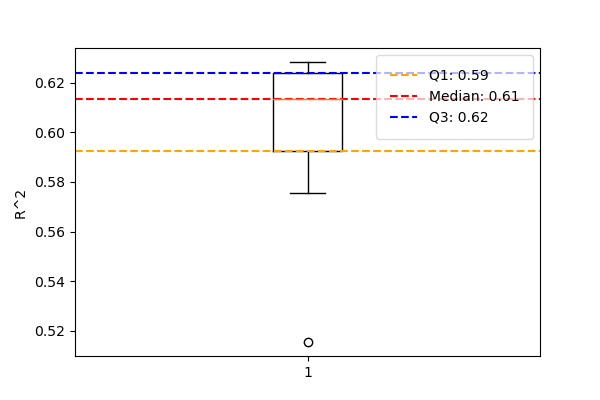
\includegraphics[width=1\columnwidth]{Images/05_results/wrench_boxplot_test_OC_R^2.png}
    \caption[\(\boldsymbol{GP}_{\text{wrench}}\) model \(R^2\) on wrench \(\mathcal{D}_{\text{CartesianOC}}\) test data]{\(\boldsymbol{GP}_{\text{wrench}}\) model \(R^2\) on wrench \(\mathcal{D}_{\text{CartesianOC}}\) test data}
    \label{fig:wrench_oc_R^2_test}
    \end{figure}

    \begin{figure}[H]
    \centering
    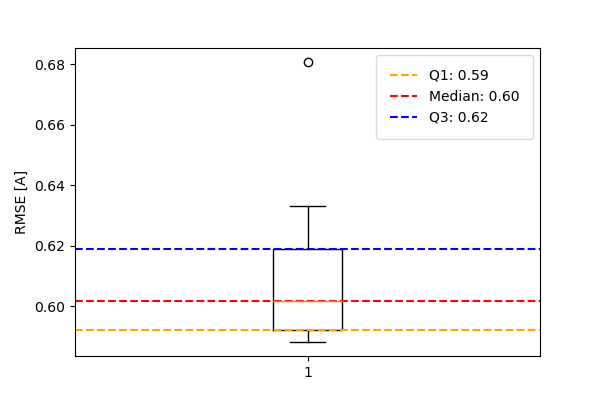
\includegraphics[width=1\columnwidth]{Images/05_results/wrench_boxplot_test_OC_RMSE.png}
    \caption[\(\boldsymbol{GP}_{\text{wrench}}\) model \(RMSE\) on wrench \(\mathcal{D}_{\text{CartesianOC}}\) test data]{\(\boldsymbol{GP}_{\text{wrench}}\) model \(RMSE\) on wrench \(\mathcal{D}_{\text{CartesianOC}}\) test data}
    \label{fig:wrench_oc_RMSE_test}
    \end{figure}
    
    \begin{table}[H]
    \centering
    \begin{tabular}{lcccc}
    \toprule
    \textbf{Model} & \textbf{MAE} & \textbf{MSE} & \textbf{RMSE} & \textbf{R\textsuperscript{2}} \\
    \midrule
    Model\_1 & 0.3196 & 0.4902 & 0.6807 & 0.5155 \\
    Model\_2 & 0.2914 & 0.4290 & 0.6331 & 0.5757 \\
    Model\_3 & 0.2798 & 0.4130 & 0.6202 & 0.5913 \\
    Model\_4 & 0.2741 & 0.4087 & 0.6152 & 0.5957 \\
    Model\_5 & 0.2688 & 0.3928 & 0.6038 & 0.6114 \\
    Model\_6 & 0.2636 & 0.3890 & 0.5993 & 0.6153 \\
    Model\_7 & 0.2588 & 0.3803 & 0.5925 & 0.6238 \\
    Model\_8 & 0.2571 & 0.3801 & 0.5921 & 0.6240 \\
    Model\_9 & 0.2541 & 0.3767 & 0.5893 & 0.6273 \\
    Model\_10 & 0.2521 & 0.3757 & 0.5882 & 0.6283 \\
    \bottomrule
    \end{tabular}
    \caption{\(\boldsymbol{GP}_{\text{wrench}}\) model metrics on effort \(\mathcal{D}_{\text{CartesianOC}}\) test data}
    \end{table}

    \begin{figure}[H]
    \centering
    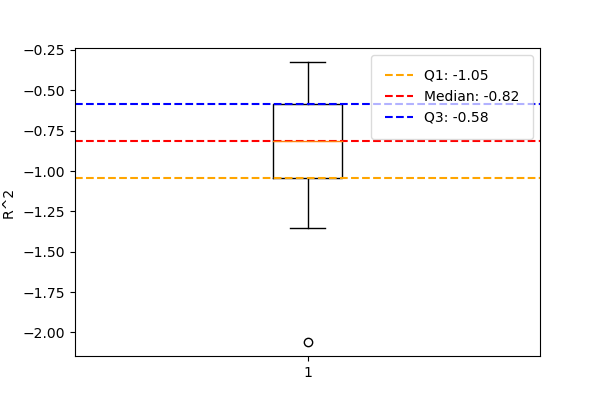
\includegraphics[width=1\columnwidth]{Images/05_results/wrench_boxplot_live_OC_R^2.png}
    \caption[\(\boldsymbol{GP}_{\text{wrench}}\) model \(R^2\) on wrench Cartesian trajectories with orientation change live prediction]{\(\boldsymbol{GP}_{\text{wrench}}\) model \(R^2\) on wrench Cartesian trajectories with orientation change live prediction}
    \label{fig:wrench_oc_R^2_live}
    \end{figure}

    \begin{figure}[H]
    \centering
    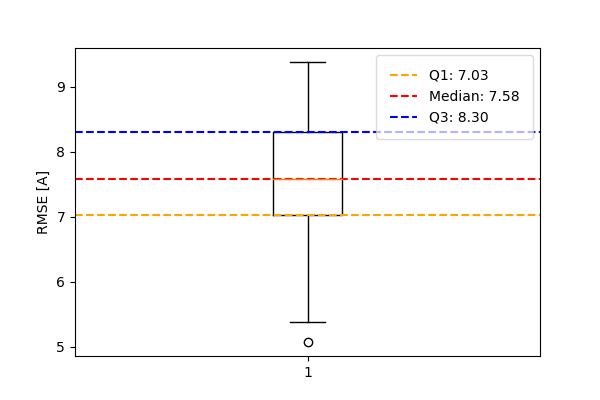
\includegraphics[width=1\columnwidth]{Images/05_results/wrench_boxplot_live_OC_RMSE.png}
    \caption[\(\boldsymbol{GP}_{\text{wrench}}\) model \(RMSE\) on wrench Cartesian trajectories with orientation change live prediction]{\(\boldsymbol{GP}_{\text{wrench}}\) model \(RMSE\) on wrench Cartesian trajectories with orientation change live prediction}
    \label{fig:wrench_oc_RMSE_live}
    \end{figure}

    
    \begin{table}[H]
    \centering
    \begin{tabular}{lcccc}
    \toprule
    \textbf{Model} & \textbf{MAE} & \textbf{MSE} & \textbf{RMSE} & \textbf{R\textsuperscript{2}} \\
    \midrule
    Model\_1 & 6.6921 & 153.0354 & 8.5885 & -2.0593 \\
    Model\_2 & 5.3542 & 111.5841 & 7.6753 & -0.3246 \\
    Model\_3 & 4.6114 & 110.5596 & 7.4602 & -0.6125 \\
    Model\_4 & 5.8744 & 138.9630 & 8.4449 & -1.0565 \\
    Model\_5 & 6.9017 & 179.3628 & 9.3817 & -1.3500 \\
    Model\_6 & 3.4584 & 48.1678 & 5.0710 & -0.4637 \\
    Model\_7 & 5.1164 & 107.0997 & 7.4934 & -0.5723 \\
    Model\_8 & 3.7980 & 53.8531 & 5.3796 & -0.6411 \\
    Model\_9 & 5.0121 & 88.8960 & 6.8829 & -1.0151 \\
    Model\_10 & 5.3321 & 125.7489 & 7.8648 & -0.9897 \\
    \bottomrule
    \end{tabular}
    \caption{\(\boldsymbol{GP}_{\text{wrench}}\) model live prediction metrics on wrench Cartesian trajectories with changing orientation}
    \end{table}


This chapter presents the experimental evaluation of the proposed hybrid semantic exploration system. Each experiment targets a specific research question and is evaluated using quantitative performance metrics.

% =====================================================================
\section{Results on Semantic Multi-Object Search Tasks}

\subsection{Experiment 1: Single-Object Success Rate (SR)}
% Add table/plot: SR across scenes (VLFM, VLMaps, OneMap, GeFF)

\subsection{Experiment 2: Navigation Efficiency (SPL)}
% Add table: SPL scores per method

\subsection{Experiment 3: Multi-Object Success Rate (MSR)}
% Compare MSR with and without hybrid fusion; baseline: OneMap, VLMaps

\subsection{Experiment 4: Ablation of Exploitation (OpenFusion)}
% MSR with OpenFusion vs. only VLFM; include error bars

% =====================================================================
\section{Experiment 5: Improving Detection Robustness via Semantic Fusion}
% Scenarios with occlusions and ambiguous detections
% FPR, semantic precision; plot fusion vs. no fusion

% =====================================================================
\section{Experiment 6: Real-World Deployment}
% Table with SR, MSR, SPL
% System monitoring: FPS, latency, CPU/GPU stats
% Qualitative discussion (figures)

\section{Experiment 7: Comparison of VL-Models for Frontier Scoring}
